\documentclass{article}
\usepackage{polski}
\usepackage[utf8]{inputenc}

\usepackage{amsthm}
\usepackage{amssymb}
\usepackage{amsmath}
\usepackage{etoolbox}
\usepackage{hyperref}
\usepackage{graphicx} %do grafik
\usepackage{float}

\graphicspath{ {obrazki/} }


\theoremstyle{definition}%
\newtheorem{defn}{Definicja}

\theoremstyle{theorem}
\newtheorem{zad}{Zadanie}
\AfterEndEnvironment{zad}{\noindent\ignorespaces}

\newtheorem{theo}{Stwierdzenie}

\renewenvironment{proof}{{\bfseries Rozwiązanie \\}}{\qed}


\title{Topologia *}
\author{Mateusz Zugaj, Michal Zmyslowski}
\date{Listopad 2017}


%Skrócone oznaczenia
\newcommand{\R}{\mathbb{R}} %Zbiór liczb rzeczywistych
\newcommand{\Pow}{\mathcal{P}} %Zbiór potęgowy
\newcommand{\sT}{\mathcal{T}} %Topologia
\newcommand{\sF}{\mathcal{F}} %Fopologia (zbiory domknięte)

\DeclareMathOperator{\id}{id} %identycznosc
\DeclareMathOperator{\cl}{cl} %domkniecie
\DeclareMathOperator{\Int}{Int} %wnętrze



\begin{document}
	
	\maketitle
	
	\section{Podstawowe przykłady topologii i ich własności.}
	
	\begin{defn}[Topologie na prostej] W zbiorze liczb rzeczywistych  $\R$ zdefiniujmy rodziny podzbiorów~${\cal T}_i$:
		\begin{enumerate}
			\item ${\cal T}_1=\Pow (\R)$ -- topologia dyskretna
			\item ${\cal T}_2=\{U\subset \R\colon  \forall_{s\in U}\exists_{t>s}[s,t)\subset U\}$ -- topologia prawej strzałki
			\item ${\cal T}_3=\{U\subset \R\colon  \forall_{s\in U}\exists_{t<s}(t,s]\subset U\}$ -- topologia lewej strzałki
			\item ${\cal T}_4=\{U\subset \R\colon  \forall_{s\in U}\exists_{r<s<t}(r,t)\subset U\}$  -- topologia euklidesowa
			\item ${\cal T}_5=\{\emptyset\}\cup\{\R\}\cup\{(-\infty,x)\colon x\in \R\}$ - topologia lewych przedziałów
			\item ${\cal T}_6=\{\emptyset\}\cup\{\R\}\cup\{(x,+\infty)\colon x\in \R\}$ - topologia prawych przedziałów
			\item ${\cal T}_7=\{\emptyset\}\cup\{\R\}\cup\{U\subset \R\colon  \R\setminus U \; \hbox{jest zbiorem skończonym}\}$ -- topologia Zariskiego
			\item ${\cal T}_8=\{\emptyset\}\cup\{\R\}$ -- topologia antydyskretna
		\end{enumerate}
	\end{defn}
	
	\begin{zad}
		Niech $\mathcal{T}_{i}$ będą rodzinami podzbiorów prostej rzeczywistej opisanymi w Definicji 1.\\
		a) Sprawdź, że rodziny $\mathcal{T}_{i}$ są topologiami.\\
		b) Porównaj topologie $\mathcal{T}_{i}$, rysując diagram inkluzji tych Topologii i zbadaj ich przecięcia.\\
		c) Zbadaj, które topologie $\mathcal{T}_{i}$ mają własność Hausdorffa.\\
		d) O których parach przestrzeni $(\mathbb{R},\mathcal{T}_{i})$,$(\mathbb{R},\mathcal{T}_{j})$ potrafisz powiedzieć, że są lub nie są homeomorficzne? Narysuj i wypełnij tabelkę.
	\end{zad}
	\begin{proof}
	b) Ewidentnie $\mathcal{T}_{2}\subset\mathcal{T}_{1}$ i $\mathcal{T}_{3}\subset\mathcal{T}_{1}$. Następnie $[0,1)\in\mathcal{T}_{2}$, ale $[0,1)\not\in\mathcal{T}_{3}$. Podobnie $(0,1]\in\mathcal{T}_{3}$, ale $(0,1]\not\in\mathcal{T}_{2}$. Mamy, że $(0,1)\in\mathcal{T}_{4}$, jak również $(0,1)\in\mathcal{T}_{3}$ i $(0,1)\in\mathcal{T}_{2}$. Jednak $[0,1)\not\in\mathcal{T}_{4}$ i $(0,1]\not\in\mathcal{T}_{4}$. Czyli $\mathcal{T}_{4}\subset\mathcal{T}_{2}$ i $\mathcal{T}_{4}\subset\mathcal{T}_{3}$. Teraz $(-\infty,1)\in\mathcal{T}_{5}$, jak również $(-\infty,1)\in\mathcal{T}_{4}$. Podobnie $(1, \infty)\in\mathcal{T}_{6}$ i $(1, \infty)\in\mathcal{T}_{4}$. Jednak $(0,1)\not\in\mathcal{T}_{5}$ i $(0,1)\not\in\mathcal{T}_{6}$. Tak więc, $\mathcal{T}_{5}\subset\mathcal{T}_{4}$ i $\mathcal{T}_{6}\subset\mathcal{T}_{4}$. Mamy $(-\infty,1)\not\in\mathcal{T}_{7}$ i $(1, \infty)\not\in\mathcal{T}_{7}$. Teraz $\mathbb{R}\setminus\{1\}\in\mathcal{T}_{7}$, ale $\mathbb{R}\setminus\{1\}\not\in\mathcal{T}_{5}$ i $\mathbb{R}\setminus\{1\}\not\in\mathcal{T}_{6}$. Jednak $\mathbb{R}\setminus\{1\}\in\mathcal{T}_{4}$. Czyli $\mathcal{T}_{7}\subset\mathcal{T}_{4}$. Ostatecznie $\mathcal{T}_{8}\subset\mathcal{T}_{5}$, $\mathcal{T}_{8}\subset\mathcal{T}_{6}$,
	$\mathcal{T}_{8}\subset\mathcal{T}_{7}$.
	c) Weźmy dowolne $x,y\in\mathbb{R}$ takie, że $x<y$. Teraz $\mathcal{T}_{1}$ ma własność Hausdorffa, bo $\{x\},\{y\}\in\mathcal{T}_{1}$. Następnie dobierzmy $s,t,r\in\mathbb{R}$, że $x\in(s,t)$ i $y\in(t,r)$. Teraz  $(s,t)\in\mathcal{T}_{4}$ i $(t,r)\in\mathcal{T}_{4}$. Więc $\mathcal{T}_{2}$, $\mathcal{T}_{3}$ i $\mathcal{T}_{4}$ mają własność Hausdorffa.
	Przestrzenie $\mathcal{T}_{i}$ dla $i=5,6,7,8$ nie mają własności Hausdorffa.\\
	d) Od razu można powiedzieć, że każda $\mathcal{T}_{i}$ dla $i=1,2,3,4$ nie jest homeomorficzna z żadną z $\mathcal{T}_{j}$ dla $j=5,6,7,8$, bo wcześniejsze mają własność Hausdorffa, a późniejsze nie. Również $\mathcal{T}_{1}$ nie jest homeomorficzna z $\mathcal{T}_{8}$, bo moc pierwszej jest większa od drugiej, co wiadomo ze Wstępu do Matematyki.
	\end{proof}
	
	\begin{zad} [Bukiet prostych] Niech $J$ będzie dowolnym zbiorem. W zbiorze $\R\times J$ rozpatrzmy relację równoważności $$(t,i)\sim (s,j)\quad\text{wtedy i tylko wtedy gdy}\quad t=s=0\quad\text{lub} \quad (t,i) = (s,j)$$ a zbiór klas abstrakcji oznaczmy  $\R\wedge J^+$. Zauważmy, że $\R\wedge J^+ = \R\times J/0\times J$ tzn. powstaje z iloczynu  $\R\times J$ przez utożsamienie do punktu podzbioru $0\times J$. W zbiorze $\R\wedge J^+$ rozpatrzymy dwie topologie:
		\begin{enumerate} 
			\item Topologię $\sT_k$ wyznaczoną przez metrykę węzła $d_k((t,i),(s,j)) = \begin{cases}  |t-s|\, \text{jeśli}\, i=j \\ |t|+|s|\, \text{jeśli}\, i\neq j\end{cases}$
			
			\item Topologię słabą $\sT_w$  tzn. taką, że zbiór $U\subset \R\wedge J^+$ jest otwarty wtedy i tylko wtedy gdy dla każdego $i\in J$ zbiór $U\cap \R\times\{i\}$ jest otwarty w topologii euklidesowej prostej. 
		\end{enumerate}
		Zauważ, że 
		\begin{enumerate}
			\item $\sT_k\subset \sT_w$
			\item Jeśli $|J|\geq \aleph_0$, to topologia słaba nie spełnia pierwszego aksjomatu przeliczalności.
			\item Jeśli $|J|\geq \aleph_0$, to topologia słaba jest niemetryzowalna.
		\end{enumerate} 
		 \end{zad}
		 \begin{proof}
		 	\begin{enumerate}
		 		\item Niech $U \in \sT_k$. Zauważmy, że kule $B((x,i),r)$ w metryce $d_k$ występują w dwóch postaciach
		 		\begin{enumerate}
		 			\item $B((x,i),r)$ dla $r\leq|x|$ jest odcinkiem otwartym na i-tej prostej, tj. \[
		 			B((x,i),r) \cap \left(\R \times {i}\right) = \underbrace{(x-r,x+r)}_{\text{przedział otwarty!}} \times \{i\}\]
		 			\begin{figure}[H]
		 			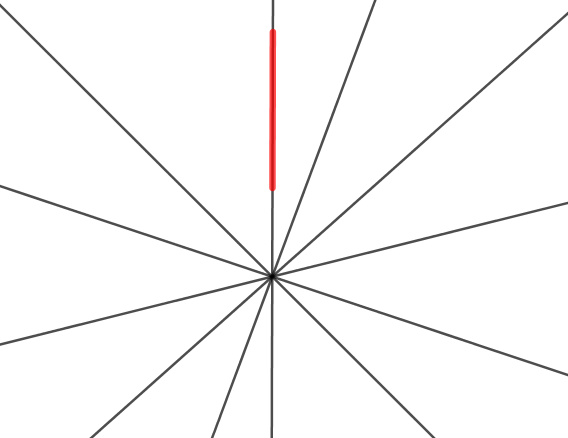
\includegraphics{zad_toposlaba1}
		 			\centering
		 			\end{figure}
		 			\item Dla $r > |x|$ jest to suma dwóch zbiorów, odcinka otwartego zdefiniowanego tak samo jak wyżej ["patyczka"] 
		 			\[
		 			B((x,i),r) \cap \left(\R \times {i}\right) = \underbrace{(x-r,x+r)}_{\text{przedział otwarty!}} \times \{i\}\]
		 			oraz zbioru ["lizaka"]
		 			\[
		 			(-(r-|x|),r-|x|)\times \left(J \setminus \{i\}\right)
		 			\]
		 		
		 	\begin{figure}[H]
		 		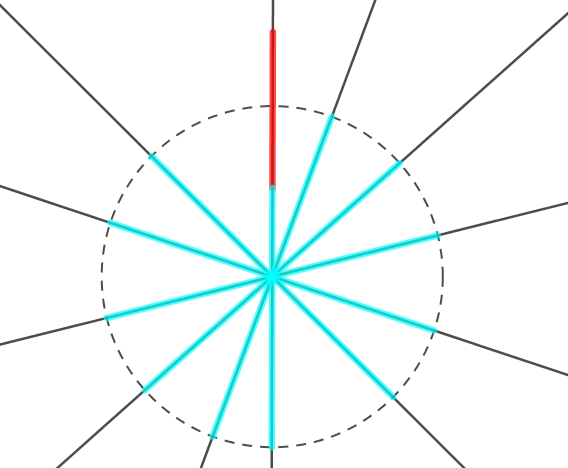
\includegraphics{zad_toposlaba2}
		 		\centering
		 	\end{figure}
		 		\end{enumerate}
		 		Z definicji przestrzeni wyznaczanej przez metrykę każdy zbiór otwarty jest sumą kul w tej metryce, tj. $U=\bigcup_{u\in U } B_u$, gdzie $B_u = B(u,r)$ są zawarte w $U$. \\
		 		Chcemy pokazać, że $U\in \sT_w$, czyli że dla każdego $i$ zbiór $U\cap \left( \R\times\{i\}\right)$ jest otwarty w topologii euklidesowej. Skoro $U = \bigcup B_u$ to wystarczy, że $B_u$ będzie otwarte w $\sT_w$ - wtedy $U$ jako suma zbiorów otwartych w $\sT_w$ będzie otwarta. \\
		 		Ale każda kula jest otwarta w $\sT_w$. Dla dowolnej zachodzi 
		 		\[
		 		B((x,j),r) \cap \left(\R \times \{i\}\right) = \begin{cases}
		 		(x-r,x+r) & r < |x| \vee j = i \\
		 		(-(r-|x|),r-|x|) & r \geq |x| \wedge j \neq i
		 		
		 		\end{cases}
		 		\]
			 	W każdym przypadku, iloczyn jest przedziałem otwartym w topologii euklidesowej. Zatem $B((x,j),r) \in \sT_w$, więc $U\in \sT_w$ zgodnie z tym co wcześniej ustaliliśmy.
			 	\item 
		 		Udowodnimy, że topologia słaba nie ma punktowej bazy przeliczalnej w 0. \\
		 		Załóżmy, że istnieje taka baza $= \{U_1,U_2,U_3,\cdots\}$. Niech $J_0 \subseteq J$ będzie zbiorem przeliczalnym w $J$ i $J_0=\{j_1,j_2,\cdots\}$. Skonstruujemy taki zbiór otwarty $U$, że $0\in V$ ale $\forall k\in \mathbb{N} \; U_k \not\subseteq V$.
		 		Mianowicie bierzemy zbiory
		 		\[
		 		V_k \subsetneq U_k \cap \left(\R \times \{j_k\}\right)
		 		\]
		 		I teraz $V=\bigcup V_k \cup \left((J\setminus J_0)\times \R\right)$. Widzimy, że gdyby $U_k \subseteq V$, to musiałoby być $U_k\cap (\R \times \{j_k\}) \subseteq V \cap (\R \times \{j_k\}) = V_k$, co jest sprzeczne z definicji $V_k$. Zatem założenie o istnieniu bazy przeliczalnej w zerze jest fałszywe.
		 		\item
		 		Gdyby przestrzeń była metryzowalna, to zbiór kul o promieniach wymiernych o środku w 0 byłaby bazą punktową przeliczalną w zerze, co przy tych założeniach jest niemożliwe na mocy poprzedniego podpunktu.
		 	\end{enumerate}
		 	
		 \end{proof}
	\section{Przestrzenie topologiczne a przestrzenie metryczne.}
	\begin{zad}
		Niech $d_i$ dla $i = 1,2$ będą dwoma metrykami w zbiorze X. Następujące warunki są równoważne:\\
		1. Topologia wyznaczona przez $d_2$ jest drobniejsza niż wyznaczona przez $d_1$, tzn. $\mathcal{T}(d_1)\subset\mathcal{T}(d_2)$.\\
		2. Dla każdej kuli $\mathcal{B}_{d_1}(x,r_1)$ istnieje liczba $r_2>0$ taka, że $\mathcal{B}_{d_2}(x,r_2)\subset\mathcal{B}_{d_1}(x,r_1)$.\\
		3. Jeśli ciąg jest zbieżny w metryce $d_2$ to jest zbieżny w metryce $d_1$ do tej samej granicy.
			\end{zad}
		\begin{proof}
		\\	$1\implies2$\\
		Załóżmy, że $\mathcal{T}(d_1)\subset\mathcal{T}(d_2)$. Niech $\mathcal{B}_{d_1}(x,r_1)\in\mathcal{T}(d_1)$. Z założenia $\mathcal{B}_{d_1}(x,r_1)\in\mathcal{T}(d_2)$. Z definicji topologii $\mathcal{T}(d_2)$ istnieje $r_2>0$ takie, że\\
		$\mathcal{B}_{d_2}(x,r_2)\subset\mathcal{B}_{d_1}(x,r_1)$.\\
		$2\implies1$\\
		Załóżmy, że  dla każdej kuli $\mathcal{B}_{d_1}(x,r_1)$ istnieje liczba $r_2>0$ taka, że\\ $\mathcal{B}_{d_2}(x,r_2)\subset\mathcal{B}_{d_1}(x,r_1)$. Weźmy dowolny $y_s\in\mathcal{B}_{d_1}(x,r_1)$. Z definicji topologii $\mathcal{T}(d_1)$ istnieje $r>0$ takie, że $\mathcal{B}_{d_1}(y_s,r)\subset\mathcal{B}_{d_1}(x,r_1)$. Z założenia istnieje $r_s>0$ takie, że $\mathcal{B}_{d_2}(y_s,r_s)\subset\mathcal{B}_{d_1}(y_s,r)$. Z tego wynika, że $\bigcup_s \mathcal{B}_{d_2}(y_s,r_s) = \mathcal{B}_{d_1}(x,r_1)\in\mathcal{T}(d_1)$. Z definicji topologii $\bigcup_s \mathcal{B}_{d_2}(y_s,r_s)\in\mathcal{T}(d_2)$. Tak, więc $\mathcal{T}(d_1)\subset\mathcal{T}(d_2)$.\\
		$1\implies3$\\
		Załóżmy, że $\mathcal{T}(d_1)\subset\mathcal{T}(d_2)$. Niech ciąg $\{x_n\}_{n=1}^\infty$ będzie zbieżny do $x$ w metryce $d_2$. Załóżmy, że $\{x_n\}_{n=1}^\infty$ nie jest zbieżny do $x$ w metryce $d_1$. Z tego wynika, że istnieje $\epsilon>0$, taki, że dla każdego $n_{\epsilon}$ istnieje $n>n_{\epsilon}$, że $x_n\not\in\mathcal{B}_{d_1}(x,\epsilon)$. Z założenia $\mathcal{T}(d_1)\subset\mathcal{T}(d_2)$ wynika jednak, że istnieje liczba $r>0$ taka, że $\mathcal{B}_{d_2}(x,r)\subset\mathcal{B}_{d_1}(x,\epsilon)$. Jako, że $\{x_n\}_{n=1}^\infty$ jest zbieżny do $x$ w metryce $d_2$, to z definicji zbieżności prawie wszystkie wyrazy $\{x_n\}_{n=1}^\infty$ znajdują się w $\mathcal{B}_{d_2}(x,r)$, co jest sprzeczne z faktem, że $x_n\not\in\mathcal{B}_{d_1}(x,\epsilon)$. Z tego wynika, że $\{x_n\}_{n=1}^\infty$ jest zbieżny do $x$ w metryce $d_1$.\\
		$3\implies1$\\
		Załóżmy, że jeśli ciąg jest zbieżny w metryce $d_2$ to jest zbieżny w metryce $d_1$. Zawieranie się topologii jest równoważne zawieraniu się rodziny zbiorów domkniętych, tzn. $\mathcal{F}_{\mathcal{T}(d_1)}\subset\mathcal{F}_{\mathcal{T}(d_2)}\Longleftrightarrow\mathcal{T}(d_1)\subset\mathcal{T}(d_2)$. Udowodnimy ten fakt w "prawą" stronę. Niech $A\in\mathcal{F}_{\mathcal{T}(d_1)}$. Jako, że $A$ jest zbiorem domkniętym to $X\setminus A$ jest zbiorem otwartym, więc $X\setminus A\in\mathcal{T}(d_1)$. Z założenia wynika, że $A\in\mathcal{F}_{\mathcal{T}(d_2)}$, więc również $X\setminus A\in\mathcal{T}(d_2)$. Niech $M\in\mathcal{F}_{\mathcal{T}(d_1)}$. Z definicji domknięcia dostajemy, że $M\subset cl_{\mathcal{T}(d_2)}(M)$. Jeżeli $x\in cl_{\mathcal{T}(d_2)}(M)$, to istnieje $\{x_n\}_{n=1}^\infty \subset M$, taki, że $d_2(x_n,x)\to 0$. Z założenia dostajemy, że $d_1(x_n,x)\to 0$. Z tego wynika, że $x\in cl_{\mathcal{T}(d_1)}(M)$. M jest domknięty w $\mathcal{T}(d_1)$, czyli $M=cl_{\mathcal{T}(d_1)}(M)$. A z tego mamy, że $x\in M$, co daje
		$cl_{\mathcal{T}(d_2)}(M)\subset M$. Wtedy $cl_{\mathcal{T}(d_2)}(M)=M$, a z tego wynika, że $M\in \mathcal{F}_{\mathcal{T}(d_2)}$, czyli  $\mathcal{F}_{\mathcal{T}(d_1)}\subset \mathcal{F}_{\mathcal{T}(d_2)}$. Tak więc, na mocy faktu, który wcześniej udowodniliśmy $\mathcal{T}(d_1)\subset\mathcal{T}(d_2)$.\\
		\end{proof}

	\begin{defn}
		Niech $(X,\mathcal{T})$ będzie przestrzenią topologiczną. Przez $C(X)$ oznaczamy zbiór
		funkcji ciągłych $f:(X,\mathcal{T}) \to (\mathbb{R},\mathcal{T}_{e})$, a przez $C_{b}(X)$ jego podzbiór składający się z funkcji ograniczonych. Dla dowolnej funkcji $f \in C_{b}(X)$ definiujemy $\|f\|_{sup}:=sup\{|f(x)|:x \in X\}$ oraz $\|f\|_{L^1}:=\int_0^1 |f(t)| dt$.
	\end{defn}
	\begin{zad}
		Porównać topologię wyznaczoną przez normę $\|f\|_{sup}$ z topologią wyznaczoną przez normę $\|f\|_{L^1}$.
	\end{zad}
	\begin{proof}
	Niech
	\[f_{n}(x):= \begin{cases} 
	1-nx\ ,\ x \in [0,\frac{1}{n}]\\
	0\ ,\ x \in (\frac{1}{n},1)
	\end{cases}\] Wtedy  $f_{n} \in C_{b}([0,1])$ i  $\|f_{n}(x)\|_{L^1}=\frac{1}{2n} \to 0$, ale
	$\|f_{n}(x)\|_{sup}=1 \not\to 0$.\\
	Rozważmy $g_{n} \in C_{b}([0,1])$ taką, że $\|g_{n}(x)\|_{sup} \to 0$.
	Wtedy na mocy \href[page=220]{skryptAM1.pdf}{9.31} $\|g_{n}(x)\|_{L^1}\leq$ $sup(|g_{n}(x)|)(1-0)\to 0$.\\
	Niech $d_{sup}(f,g)=\|f-g\|_{sup}$ i $d_{L^1}(f,g)=\|f-g\|_{L^1}$.
	Rozpatrzmy $(C_{b}(X), d_{sup})$  i $(C_{b}(X), d_{L^1})$. Jeżeli $f_n$ jest zbieżny do f w przestrzeni $(C_{b}(X), d_{sup})$, tzn. $d_{sup}(f_n,f)\to0$, to z wcześniejszych obserwacji $d_{L^1}(f_n,f)\to0$, czyli jest zbieżny, również do f, w $(C_{b}(X), d_{L^1})$. Z poprzedniego zadania wiemy już, że wtedy $\mathcal{T}(d_{L^1})\subset\mathcal{T}(d_{sup})$.
	\end{proof}
	\section{Konstrukcje topologiczne.}
	\subsection{Iloczyn topologii.}
	\begin{zad}
		Wykaż, że dla dowolnych przestrzeni $(X,\sT_X)$, $(Y,\sT_Y)$,$(X_i,\sT_{X_i})_{i\in I}$ podzbiorów $A\subseteq X$, $B\subseteq Y$ i rodzin podzbiorów $\mathcal{A}=\{A_i \mid A_i\subseteq X_i\}$ zachodzi 
		\begin{enumerate}
			\item $\Int(A\times B)=\Int(A)\times \Int(B)$
			\item $\Int(\prod \mathcal{A}) \subseteq \prod \{\Int(A_i) \mid A_i \in \mathcal{A}\}$, + kontrprzykład braku zawierania w drugą stronę
			\item $\cl(A\times B) = \cl(A) \times \cl(B)$
			\item $\cl(\prod \mathcal{A}) = \prod \{\cl(A_i) \mid A_i \in \mathcal{A} \}$
		\end{enumerate}
	
	\end{zad}
	\begin{proof}
		\begin{enumerate}
			\item 
			$\subseteq$: Niech $x\in \Int(A\times B)$. Skoro tak, to istnieje otwarte otoczenie $U \ni x$ i $U \subseteq A\times B$, z definicji wnętrza. Teraz użyjemy faktu, że rzutowania na współrzędne $p_X$ oraz $p_Y$ są \emph{otwarte}, tj. obrazy zbiorów otwartych w tych przekształceniach są otwarte. [\href[page=42]{topologia_star_I_2017Z.pdf}{Wniosek 5.4.1}] \\
			Zatem $p_X(x)\in p_X[U] \in \sT_X$, co dowodzi że $p_X(x)\in \Int(A)$, gdyż $p_X[U]\subseteq A$ jest otwartym otoczeniem $x$. Analogiczne $p_Y(x)\in \Int(B)$. Zatem
			\[
		x=	(p_X(x),p_Y(x)) \in \Int(A)\times \Int(B)
			\]
			\\
			$\supseteq$: Niech $(x,y) \in \Int(A)\times \Int(B)$, czyli $x\in \Int(A) \wedge y\in \Int(B)$. W takim razie istnieją dwa otoczenia, $U_x \ni x$, $U_y \ni y$ i dostajemy
			\[
			(x,y) \in p_X^{-1}[U_X] \cap p_Y^{-1}[U_Y] 
			\] 
			przy czym prawa strona jest otwarta jako przecięcie dwóch zbiorów otwartych.
			\item
			Dowód na zawieranie w prawą stronę pozostaje w większości taki sam jak w przypadku skończonym, wystarczy uwzględnić nieskończoność; że dla każdego $i\in I$ mamy $p_i[U] \in \sT_{X_i}$ i wtedy
			\[
			p_1(x)\in p_1[U],p_2(x) \in p_2[U], p_3(x) \in p_3[U], \dots 
			\]
			zatem mamy
			\[
				p_1(x)\in \Int(A_1),p_2(x) \in \Int(A_2), p_3(x) \in \Int(A_3), \dots 
			\]
			czyli z tego wynika
						\[
						x=(p_1(x),p_2(x),\dots) \in \Int(A_1)\times \Int(A_2) \times \dots = \prod \{\Int(A_i) \mid A_i \in \mathcal{A}\} 
						\]
			\\
			W drugą stronę dowód upada w momencie przecięcia przeciwobrazów - przecięcie nieskończonej liczby zbiorów otwartych \textbf{nie musi} być otwarte. \\
			Niech $\forall i\in I \; X_i = \R$. Udowodnimy, że 
			\[
			\Int\left(\prod_{i=0}^{\infty} (0,1) \right) = \varnothing
			\]
			czyli że zbiór pod operatorem wnętrza nie jest otwarty. Gdyby był otwarty, to zawierałby zbiór z bazy standardowej (tj. z [\href[page=42]{topologia_star_I_2017Z.pdf}{Stwierdzenia 5.4.1 (2)}]) gdzie, jak widzimy, jest napisane że 
			\[
			U_i = Y_i ( = \R ) \text{ dla } i \text { poza  pewnym skończonym zbiorem indeksów }
			\]
			innymi słowy, w takim iloczynie pojawi się nieskończenie wiele $\R$; w szczególności pojawi się na co najmniej raz: \[{U_1\times U_2\times\dots} \times \R \times U_{i+1} \times \dots \subseteq \prod_{i=0}^{\infty}(0,1)\]
			co jest sprzecznością, gdyż prawa strona nie zawiera $\R$ na żadnej współrzędnej.
			\item
			analogiczne
			\item
			analogicznie, tylko teraz nieskończenie przecięcie zbiorów domkniętych \textbf{już jest} zbiorem domkniętym
		\end{enumerate}
		\begin{zad}
			Przestrzeń topologiczna $(X, \sT_X )$ jest przestrzenią Hausdorffa wtedy i tylko wtedy gdy przekątna
			jest podzbiorem domkniętym produktu $(X, \sT_X ) \times (X, \sT_X )$.
		\end{zad}
		\begin{proof}
			$\Rightarrow$ \\
			Udowodnimy, że $\Delta = \{(x,x) \mid x\in X \}$ jest podzbiorem domkniętym, czyli że $(X\times X) \setminus \Delta$ jest podzbiorem otwartym. Aby to zrobić, weźmiemy punkt spoza przekątnej i pokażemy, że istnieje jego otwarte otoczenie nieprzecinające jej.\\
			Niech $(x,y) \notin \Delta$, czyli $x\neq y$. Ale mamy przy tym $x,y\in X$, czyli \emph{działa własność Hausdorffa}, mianowicie istnieją otwarte otoczenia $U_x \ni x$ oraz $U_y \ni y$ zawarte w $X$, że $U_x \cap U_y = \varnothing$. Teraz bierzemy
			\[
			U_x \times U_y \in (x,y)
			\]
			Jest to zbiór otwarty, gdyż można go zapisać jako
			\[
			p_X^{-1}[U_x] \cap p_X^{-1}[U_y]
			\]
			czyli przecięcie dwóch zbiorów otwartych - więc otwarte. Ponadto, ten zbiór jest rozłączny z przekątną, gdyż
			\begin{equation}\label{hausdiago}
			(z,z)\notin U_x \times U_y \Leftrightarrow z \notin U_x \wedge z \notin U_y \Leftrightarrow z \notin U_x \cap U_y \Leftrightarrow U_x \cap U_y = \varnothing
			\end{equation}
			jednak wiemy już, że $U_x \cap U_y = \varnothing$.\\
			$\Leftarrow$ \\
			Dowód powyżej składał się prawie cały z równoważności; po prostu aby znaleźć dwa rozłączne otoczenia punktów $x,y\in X$ (tym samym udowodnić własność Hausdorffa) wystarczy że weźmiemy otwarte otoczenie punktu $(x,y)\in X\times X$ nieprzecinające przekątnej (która jest domknięta, więc zawsze się takie znajdzie) a następnie zrzutować je na obie osie. Te dwa obrazy będą rozłączne \eqref{hausdiago}, czyli to kończy nasze poszukiwania.
			
		\end{proof}
	\end{proof}
	\subsection{Iloraz topologii.}
	\begin{defn}
		Odwzorowanie $f:(X,\sT_X) \to (Y,\sT_Y)$ nazywa się \emph{ilorazowe} jeśli jest
		\begin{itemize}
			\item surjekcją
			\item ciągłe
			\item zachodzi implikacja: jeśli przeciwobraz $f^{-1}[V]$ podzbioru $V\subset Y$ jest otwarty w $(X,\sT_X)$, to $V$ jest otwarty w $(Y,\sT_Y)$.\\
			Mówimy, że przekształcenie spełniające tę implikację jest \emph{dzielne}.
		\end{itemize}
		Innymi słowy, implikacja definiująca odwzorowania ciągłe (\emph{jeśli $V$ otwarte to $f^{-1}[V]$ otwarte}) staje się równoważnością.
	\end{defn}
	
	\begin{zad}\label{equiv_quotient_maps}
		Dla ciągłej surjekcji $f:(X,\sT_X)\to(Y,\sT_Y)$ następujące warunki są równoważne:
		\begin{enumerate}
			\item $f$ jest przekształceniem ilorazowym
			\item 	$\forall V\subset Y \quad V \in \sT_Y \Longleftrightarrow f^{-1}[V] \in \sT_X$
			\item $\forall B\subset Y \quad B \in \sF_Y \Longleftrightarrow f^{-1}[B] \in \sF_X$ 
			\item $\sT_*(\{f\})=\sT_Y$
		\end{enumerate}
		
	\end{zad}
	\begin{proof} 
		\emph{1} $\implies$ \emph{2} \\
		Prosto z definicji, ta równoważność to ciągłość i dzielność jednocześnie. \\
		\emph{2} $\implies$ \emph{1} \\
		Oczywiście są spełnione wszystkie warunki z definicji przekształcenia ilorazowego - bycie surjekcją jest zapewnione z treści zadania, a ciągłość i dzielność jednocześnie to nasze założenie.
		\\
		\emph{2} $\implies$ \emph{3} \\
		Załóżmy \emph{2}. Musimy pokazać równoważność $B \in \sF_Y \Leftrightarrow f^{-1}[B]$ dla każdego podzbioru $B\subset Y$. \\
		 Niech $B\in \sF_Y$. To znaczy, że $Y\setminus B \in \sT_Y$. Ale wtedy $f^{-1}[Y\setminus B] \in \sT_X$, z założenia \emph{1}. Ale zachodzi tożsamość przeciwobrazów \[f^{-1}[Y\setminus B] = f^{-1}[Y]\setminus f^{-1}[B]\] [Guzicki, Zakrzewski, Twierdzenie 3.16 (8)]. Oczywiście $f^{-1}[Y] = X$, zatem dostajemy $f^{-1}[Y\setminus B] = X \setminus f^{-1}[B] \in \sT_X$, a więc $f^{-1}[B] \in \sF_X$.
		 \\
		Każde wynikanie powyżej było tak naprawdę równoważnością, włącznie z założeniem \emph{1}. Zatem równoważność jest udowodniona.
		\\
		\emph{3} $\implies$ \emph{2}
		\\
	Dowód identyczny jak powyżej, wystarczy $\sT$ i $\sF$ zamienić miejscami.
	\\
	\emph{2} $\implies$ \emph{4}
	\\
	Wiemy, że $\sT_*(\{f\})=\{V\subseteq Y \mid f^{-1}[V]\in \sT_X \} $, więc musimy udowodnić, że \[
	\{V \subseteq Y \mid f^{-1}[V] \in \sT_X \} = \sT_Y
	\]
	$\subseteq$: Niech $U \in \{V \subset Y \mid f^{-1}[V] \in \sT_X \}$. Zatem $f^{-1}[U] \in \sT_X$. Z ze strony $\Leftarrow$ implikacji \emph{2} mamy $U \in \sT_Y$. To dowodzi zawierania w lewą stronę. \\
	$\supseteq$: Niech $U \in \sT_Y$. Zatem ze strony $\Rightarrow$ implikacji \emph{2} mamy $f^{-1}[U] \in \sT_X$. Z definicji dostajemy $U \in \{V \subset Y \mid f^{-1}[V] \in \sT_X \}$.
	\\
	\emph{4} $\implies$ \emph{1}
	\\
	To, że $f$ jest surjekcją mamy z treści zadania. $f$ jest również ciągła w $\sT_Y$ z definicji $\sT_*$.\\
	Pozostaje udowodnić dzielność. Kluczowym faktem tutaj jest to, że $\sT_*(\{f\})$ jest \emph{największą} topologią taką, że $f$ jest ciągłe. Gdyby $f^{-1}[V] \in \sT_X \not\Rightarrow V \in \sT_Y$ to istniałaby topologia $\sT_Y' = \sT_Y \cup \{V\}$ ściśle większa od $\sT_Y$ dla które $f$ nadal byłoby ciągłe, gdyż $V\in \sT_Y'$ i $f^{-1}[V] \in \sT_X$. Sprzeczność. Zatem $f$ jest dzielne.
	
	\end{proof} 
	\begin{defn}
		Przekształcenie ciągłe $f:(X,\sT_X) \to (Y,\sT_Y)$ nazywamy \emph{otwartym} (\emph{domkniętym}) jeśli obraz dowolnego zbioru otwartego (domkniętego) w $(X,\sT_X)$ jest otwarty (domknięty) w $(Y,\sT_Y)$.
	\end{defn}
	\begin{zad}
		Jeśli $f: (X,\sT_X) \to (Y,\sT_Y)$ jest otwartą lub domkniętą ciągłą surjekcją, to $f$ jest przekształceniem ilorazowym. 
	\end{zad}
	\begin{proof}
		Ciągłość i surjektywność mamy z treści zadania. Pozostaje sprawdzić
		\[
		f^{-1}[V]\in \sT_X \implies V \in \sT_Y
		\]
		Załóżmy, że $f^{-1}[V] \in \sT_X$. Jeśli $f$ jest otwarte, to znaczy że $f[f^{-1}[V]] \in \sT_Y$. Ale $f[f^{-1}[V]] = V$ [Guzicki, Zakrzewski, Twierdzenie 3.15 (3)], zatem $V\in \sT_Y$.
		\\
		W przypadku, kiedy $f$ jest domknięte korzystamy z równoważnego warunku udowodnionego w zadaniu \ref{equiv_quotient_maps}:
		\[
		f^{-1}[B]\in \sF_X \implies B \in \sF_Y
		\]
	\end{proof}
	\begin{defn}
		 Jeśli $A\subset X$ jest podzbiorem przestrzeni topologicznej $(X,\sT_X)$ to przez $X/\{A\}$  lub $X/A$ oznaczamy \emph{przestrzeń ilorazową} relacji równoważności takiej, że $x \sim y\, \iff \, x=y$ {lub}\, $x,y\in A$ z topologią popchniętą przez projekcję $p: X \to X/A$, $p(x)=p(y) \Leftrightarrow x \sim y$.
	\end{defn}
	\begin{zad}
		Jeśli $A\subset X$ jest podzbiorem domkniętym (otwartym), to projekcja $p\colon X\to X/A$ jest odwzorowaniem domkniętym (otwartym).
	\end{zad}
	\begin{proof}
		
		Niech $A \in \sF_X$ i skoro $\forall x,y \in A \quad p(x)=p(y) =: a$ to mamy $\{a\}=p[A]$. Zgodnie z definicją [\href[page=40]{topologia_star_I_2017Z.pdf}{Definicja 5.3.1}] mamy (zamieniając zbiory otwarte na domknięte)
		\[
		\sF_{X/A} = \{B\subset X/A \mid p^{-1}[B] \in \sF_X \}
		\]
		Niech $B_0 \in \sF_X$. Musimy udowodnić, że $p[B_0]\in \sF_{X/A}$. Na mocy definicji powyżej, to jest równoważne udowodnieniu 
		\[
		p[B_0]=B, \text{ takie że } p^{-1}[B]\in \sF_X
		\]
		Czyli, innymi słowy
		\[
		p^{-1}[p[B_0]]\in \sF_X
		\]
		Nie zachodzi w ogólności równość; $C \neq f^{-1}[f[C]]$, nie wystarczy to do udowodnienia powyższego należenia. \\
		
				Musimy rozważyć dwa przypadki:
	

		\begin{enumerate}
			\item $B_0 \cap A = \varnothing$ \\
			Wtedy $p^{-1}[p[B_0]]=B_0$, dlatego bo $p|_{X\setminus A} = \id$. Zatem
			\[
			p^{-1}[p[B_0]]=B_0\in \sF_X
			\]
			\item $B_0 \cap A \neq \varnothing$ \\
				Zachodzą następujące równości: \[(B_0 \setminus A) \cap A = \varnothing\] oraz \[
				(B_0 \setminus A) \cup (B_0 \cap A) = B_0
				\]
				Używając też związku $p[C\cup D] = p[C] \cup p[D]$ [Tw. 3.16 (3)] dostajemy
				\[
				p[B_0]=p[(B_0 \setminus A) \cup (B_0 \cap A)] = p[B_0 \setminus A] \cup p[B_0 \cap A] 
				\]
				Skoro $p|_{X\setminus A} = \id$, to $p[B_0\setminus A] = B_0\setminus A$.
				$B_0\cap A$ to podzbiór $A$, zatem $p$ na każdym elemencie tego zbioru będzie wynosiło $a$, z definicji projekcji. Mamy zatem
				\[
				 p[B_0 \setminus A] \cup p[B_0 \cap A]  = (B_0\setminus A) \cup \{a\}
				\]
				Teraz używając związku $p^{-1}[C\cup D] = p^{-1}[C] \cup p^{-1}[D]$ [Tw. 3.16 (6)] mamy
				\[
				p^{-1}[p[B_0]] = p^{-1}[(B_0\setminus A)\cup \{a\}] = p^{-1}[B_0\setminus A]\cup p^{-1}[\{a\}] = (B_0\setminus A) \cup A = B_0 \in \sF_X
				\]
		\end{enumerate}
		
		Dla przypadku otwartego, każdy symbol $\sF$ w dowodzie powyżej należy zastąpić symbolem $\sT$; dowód jest po prostu analogiczny.
	\end{proof}
	\begin{zad}
		Podaj przykład odwzorowania ilorazowego, które nie jest ani domknięte, ani otwarte.
	\end{zad}
	\begin{proof}
		
		Patrząc na wcześniejsze zadanie wystarczy dojść do wniosku, że jeśli $A$ nie jest ani otwarte, ani domknięte to nie możemy udowodnić otwartości lub domkniętości $p$. Wykorzystamy to. \\
		Niech $X=\R$ z topologią euklidesową $\sT_e$. Niech $A = [0,1)$. Bierzemy przestrzeń $X/A$ z zadaną projekcją
		\[
		p(x) = \begin{cases}
		x & x \notin [0,1) \\
		a & x \in [0,1)
		\end{cases}
		\]
		gdzie $a=[0]$, czyli klasa abstrakcji zera; mianowicie punkt do którego został \textit{zwinięty} przedział $[0,1)$.
		$p$ jest przekształceniem ilorazowym jako przekształcenie które zadaje przestrzeń ilorazową zgodnie z zadaniem \ref{equiv_quotient_maps}. \\
		Jednak $p$ nie jest otwarte ani domknięte. Zacznijmy od tego, że $\{a\} \notin \sT_{X/A}$ ani $\{a\} \notin \sF_{X/A}$, gdyż $p^{-1}[\{a\}] = A=[0,1) \notin \sT_{(X/A)} \cup \sF_{(X/A)}$.
		Mamy z tego
		\[
		\left[\frac14,\frac12\right] \in \sF_X \wedge p\left[\left[\frac14,\frac12\right]\right]=\{a\} \notin\sF_{X/A}\text{, czyli } p\text{ nie jest domknięte}
		\]
		\[
		\left(\frac14,\frac12\right) \in \sT_X \wedge p\left[\left(\frac14,\frac12\right)\right]=\{a\}\notin \sT_{X/A}\text{, czyli } p\text{ nie jest otwarte}
		\]
	\end{proof}
\end{document}